\chapter{Realisierung Objekt Erkennung}\label{kap:objerk}

\section{Datensatz}\label{sec:dataset}

Um ein Deep Learning Modell vernünftig trainieren zu können, 
wird eine große Menge an gelabelten Trainingsdaten benötigt.
Im Falle der Objekterkennung enthalten die labels neben der 
Klasse auch die Koordinaten der Bounding Boxen.


Für die vorliegende Arbeit wurden dafür aus dem Open Source 
Dataset \textit{OpenImages} \cite{kuznetsovaOpenImagesDataset2018} 
von Google 9 Klassen die Wildtiere enthalten heruntergeladen.

Dieses besteht aus einem Trainingsset mit 200 bis 2000 Bildern pro 
Klasse sowie einem Test- und einem Validierungsset. Um für alle Klassen 
die gleiche Anzahl an Trainingsdaten zu erhalten und um Overfitting zu 
verhindern wurden wie im folgenden beschrieben die Trainingsdaten 
augmentiert.

\subsection{Augmentierung}

Augmentierung ist eine Technik aus den vorhandenen Daten 
künstlich mehr Daten zu generieren, indem diese leicht 
abgeändert werden. Im Falle des für diese Arbeit verwendeten
OpenImages Datensatzes wurden Geometrische Transormationen 
wie Sklierung, Verschiebung Rotieren oder Spiegeln und 
Manipulationen der Pixelwerte wie ändern der 
Farbwerte, Helligkeit, Kontrast oder Rauschen vorgenommen.

\begin{figure}[htb]
    \centering
    \label{fig:augmentierung}
    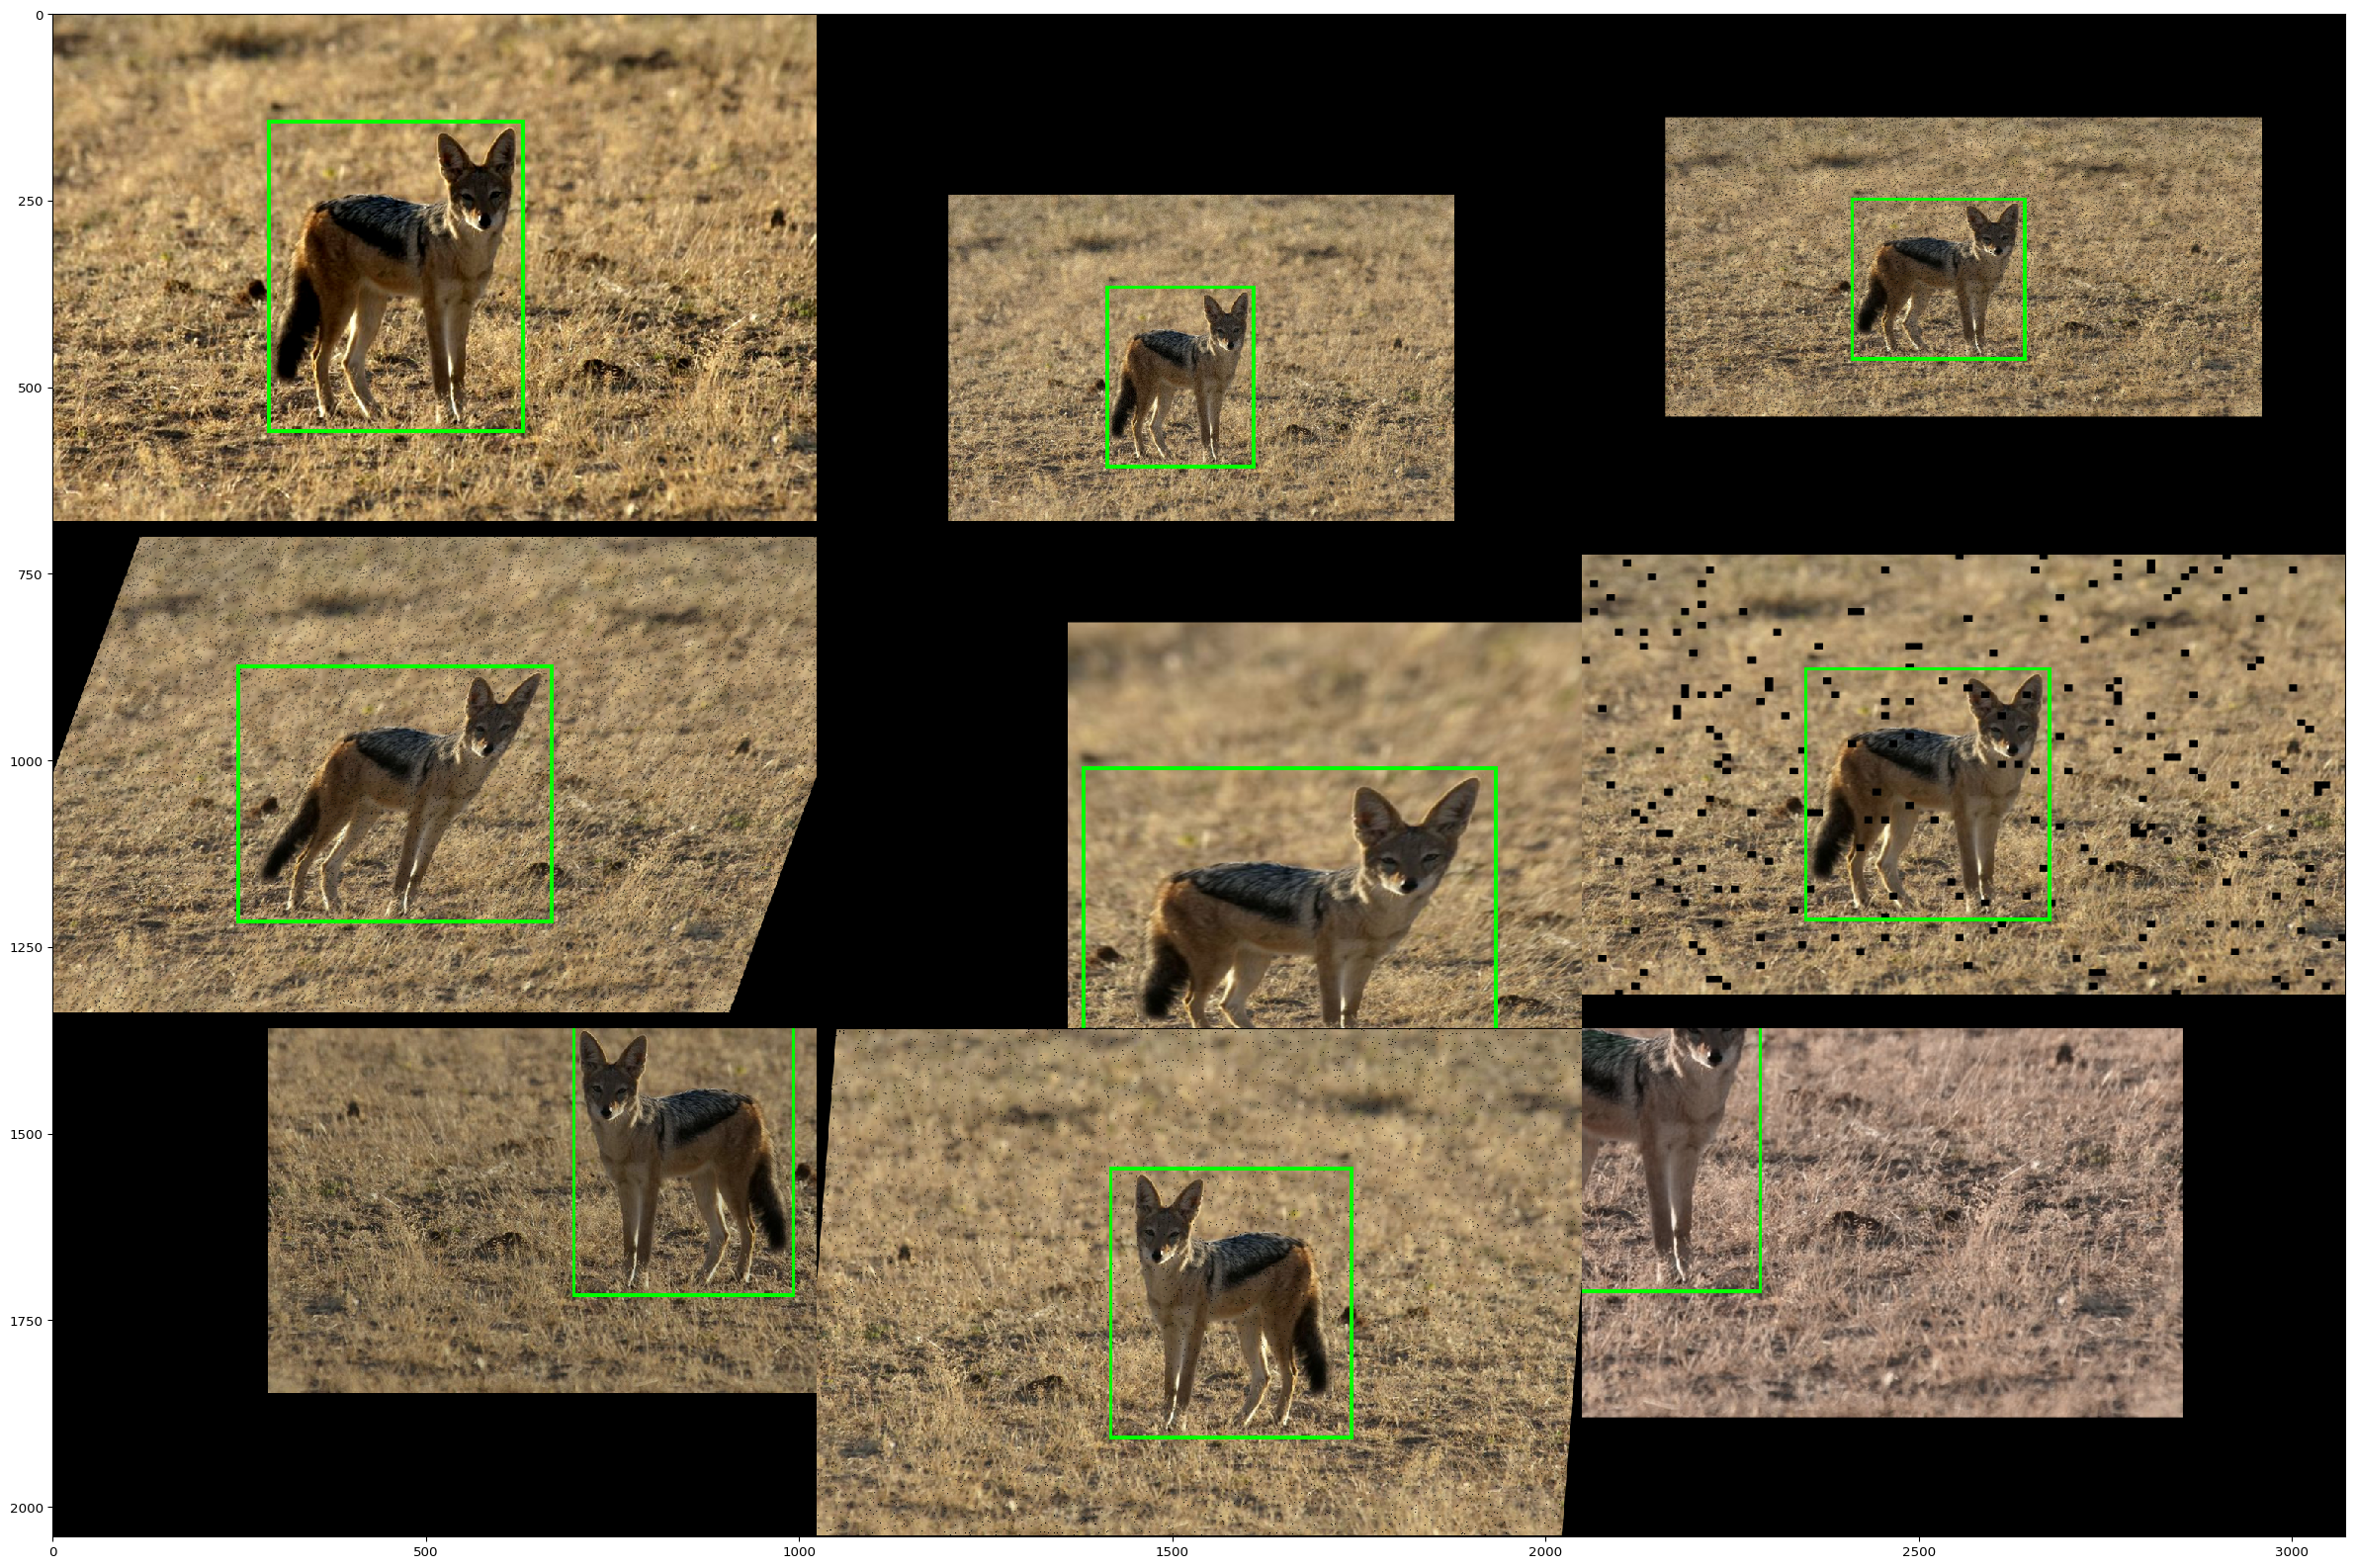
\includegraphics[width=0.8\columnwidth]{Bilder/augmentierung.png}
    \caption{Anwendung von Augmentierungstechniken}
\end{figure}


\section{Training}

Da der Neural Compute Stick mit OpenVino ein eigenes Datei Format 
für die traininerten Modelle verwendet, musste bei der Auswahl
eines Frameworks sowie Models auf die Kompatibilität zu OpenVino 
geachtet werden. 

Verwendete wurde daher das untersstütze Framework Tensorflow, 
um zwei Ansätze zu verfolgen. Der eine verwendet die Api Keras, 
und versucht neben der Klassifikation die Lokalisierung mit 
dieser vorzunahemen, der andere verwendet eine speziell für die 
Objekterkennung konzipierte Api für wie in Abschnitt
 \ref{sec:related_work} beschriebene End-to-End lösungen.

\subsection{Tensorflow Object Detection Api}

Die Tensorflow Object Detection Api ist unter den Research Modellen
\cite{HttpsGithubCom} des offiziellen Tensorflow Repository zu
finden und enthällt implementierungen einiger gängiger Object Detectin
Modelle, wie Single Shot Detectors (SSD) und Faster R-CNNs mit 
verschiedenen Basis CNNs mit vortrainierten Geweichten.

Um die Modelle trainieren zu können, mussten zunächst die 
Trainingsdaten in das binary Dateiformate TFRecords umgewandelt 
werden, welches die Api verwendet. Dieses ist eine Serialisierte 
darstellung der Daten als Protocol Buffer für effiziente Zufriff.



\subsection{Regularisierung}

Um das Overfitting zu vermeiden gibt es wie in \ref{sec:nn} 
beschrieben vershiedene Möglichkeiten.

Untersucht wurde hier

\begin{itemize}
    \item Augmentierung
    \item Early Stopping
    \item \dots weitere zB $L_{1}$, $L_{2}$
\end{itemize}



\subsection{Training grayscale}\label{subsec:train_gray}

Da die Kamera im Infrarot Modus ein Graustufen Bild mit nur einem 
Farbchannel liefert, muss dies für die Inferenz berücksichtigt werden.

Es ergeben sich hier mehrere möglichkeiten:

\begin{enumerate}
    \item Normales (r, g, b) Netz
    \item Ein Farbchannel (gr) Netz
    \item Drei Farbchannel (gr, gr, gr)
\end{enumerate}

Für 1. und 3. Müssen die bilder der Kamera vor der 
Inferenz auf 3 Farbchannel ($3 \times grau$) erweitert werden.
\\
Um das Netz auf einen Channel zu trainieren wurde im config file \dots
\\
Um $3 \times gray$ zu trainieren wurden die Bilder in OpenCV in 
grau convertiert und wieder als jpgs abgespeichert.

Die Ergebnisse sind in Kapitel \ref{kap:eval} dargestellt.


\section{Parameter Optimierung}
einstellungen im Config File\\
tensorflow graph oder plot zeigen\\
loss erklären (mit formel und für train und eval)


